\documentclass{article}
\usepackage{graphicx}
\usepackage{amsmath}
\usepackage{amssymb}
\usepackage{enumitem}
\usepackage{hyperref}

\begin{document}
\title{Lista de Exercícios 1 - Cálculo 2}
\author{Débora D'Angelo Reina de Araujo}
\date{\today}

\maketitle

\begin{enumerate}
    \item Mostre que as curvas regulares $\alpha(t) = (t, e^t), t \in \mathbb{R}$ e $\beta(s)=(log(s),s),s \in (0, \infty)$ têm o mesmo traço. \\
    
    \begin{figure}[!htb]
        \centering 

        \begin{subfigure}{\textwidth} % Imagem 1
            \centering
            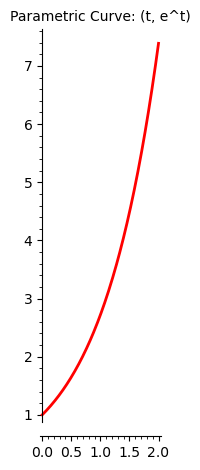
\includegraphics[width=0.3\linewidth]{imgs/curve1.png} % Substitua 'imagem1' pelo nome do seu arquivo
            \label{fig:imagem1}
        \end{subfigure}
        \begin{subfigure}{\textwidth} % Imagem 2
            \centering
            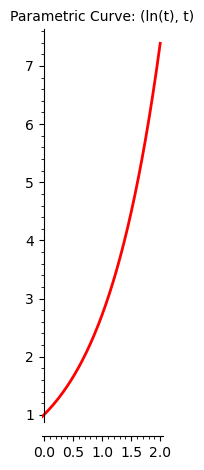
\includegraphics[width=0.3\linewidth]{imgs/curve2.png} % Substitua 'imagem2' pelo nome do seu arquivo
            \label{fig:imagem2}
        \end{subfigure}
        \label{fig:exemplo_duas_imagens} % Rótulo para referenciar no texto
    \end{figure}

    Podemos reparametrizar $alpha$ para $beta$ usando a função $\phi(t) = ln(s)$. 

    Assim $\alpha(\phi(t)) = \beta(s) = (ln(s), s)$.

    Analogamente temos $\psi(s) = e^t$ tal que $\beta(\psi(s)) = \alpha(t) = (t, e^t)$.

    Sendo $\phi$ bijetora $((0, \infty)) \to \mathbb{R}$ e $\psi$ bijetora ($\mathbb{R} \to (0, \infty)$), deriváveis e com derivadas sempre não nulas.

    Logo, possuem o mesmo traço.

    \item \textbf{(Importante!)} Calcule o comprimento de arco das seguintes curvas:
    \begin{enumerate}[label=(\alph*)]
        \item $\alpha(t) = (3cosh2t, 3sinh2t, 6t), t \in [0, pi]$ \\
        \\
        $\alpha'(t) = (6sinh(2t), 6cosh(2t), 6) $ \\
        $||\alpha'(t)|| = 6\sqrt{cosh^2(2t) + sinh^2(2*t) + 1} = 6\sqrt{cosh{4t} + 1} $ \\
        $\int_{0}^{\pi} ||\alpha'(t)|| dt = \int_{0}^{\pi} 6\sqrt{cosh{4t} + 1} dt $\\
        $\int_{0}^{\pi} ||\alpha'(t)|| dt = \frac{3}{2} (\sqrt{2}e^{2t} - \sqrt{2}e^{-2*t})|_{0}^{pi} \approx 1135,945 $
        \\
        \item Catenária: $\gamma(t) = (t, cosh(t))$, a partir do ponto (0, 1).\\
        \\
        $\alpha'(t) = (1, sinh(t))$ \\
        $||\alpha'(t)|| = \sqrt{sinh(t)^2 + 1} $ \\
        $\int_{0}^{1} ||\alpha'(t)|| dt = \frac{1}{2} (e^{t} - e^{-t})|_{0}^(1) \approx 1.175 $
    \end{enumerate}

    \item \textbf{(Importante!)} Mudanças de parâmetro:
    \begin{enumerate}[label=(\alph*)]
        \item Demonstrar que $s(\theta) = \frac{\theta^{2}}{\theta^{2} + 1}$ é uma mudança de parâmetro diferenciável que transforma o intervalo $(0, \infty)$ no intervalo $(0, 1)$ \\
        \\
        A função $s(\theta)$ é um polinômio com denominador e numerador diferenciáveis, e denominador maior que 0 para qualquer $\theta \geq 0$. Logo é diferenciável. \\
        $s'(\theta) = \frac{2t}/{(t^{2} + 1)} - \frac{2t^{3}}/{(t^2 + 1)^{2}} $ \\
        \\
        $ \lim_{\theta \to 0} s(\theta) = \lim_{\theta \to 0} \frac{\theta^{2}}{\theta^{2} + 1} = \frac{0^{2}}{0^{2} + 1} = 0 $ \\
        $ \lim_{\theta \to \infty} s(\theta) = \lim_{\theta \to \infty} \frac{\theta^{2}}{\theta^{2} + 1} = \lim_{\theta \to \infty} \frac{\frac{\theta^{2}}{\theta^{2}}}{\frac{\theta^{2}}{\theta^{2}} + \frac{1}{\theta^{2}}} = \frac{1}{1+0} = 1 $ \\
        Portanto $s$ leva o intervalo $(0, \infty)$ para $(0, 1)$.
        \\
        \item Mostrar que a função $\lambda : (-1, 1) \to (-\infty, +\infty)$ definita por $\lambda(t) := tan(\pi t/2)$ é uma mudança de parâmetro. \\
        \\
        A função $\lambda$ é derivável com valor $\lambda'(t) = \frac{\pi}{2} sec^{2}(\frac{\pi t}{2})$. \\
        \\
        $ \lim_{t \to -1} \lambda(t) = \lim_{t \to -1} tan(\pi t/2) = -\infty $ \\
        $ \lim_{t \to 1} \lambda(t) = \lim_{t \to 1} tan(\pi t/2) = +\infty $ \\
        Portanto $\lambda$ leva o intervalo $(-1, 1)$ para $(-\infty, +-\infty)$.
        \\
        \item Provar que qualquer curva pode ser reparametrizada de forma tal que o domínio da reparametrização seja um intervalo de extremos 0 e 1. \\
        \\
        Vamos chamar de L o cumprimento de uma curva regular $\alpha: [a, b] \to \mathbb{R}$. \\
        $$ L = \int_{a}^{b} ||\alpha'(t)|| dt $$
        Vamos criar uma função de reparametrização $\phi$ de modo que $\phi(t)$ mede a proporção de comprimento percorrido de $[a, t]$, com $a \leq t \leq b$. \\
        $$ \phi(t) = \frac{1}{L} \int_{a}^{t} ||\alpha'(t)|| dt $$
        A funçao $\phi$ é diferenciável porque é a integral de funções contínuas, $\phi(0) = 0$ e $\phi(b) = 1$ logo $\phi$ leva o intervalo $[a, b]$ para $[0, 1]$.
    \end{enumerate}
    \item Provar que a curva $$ \gamma(t) = (2t, \frac{2}{1+t^2}) $$ com $t > 0$ é regular e é uma reparametrização de $$ \alpha(t) = (\frac{2cos(t)}{1+sin(t)}, 1+sin(t)), \hspace{1cm} t \in (-\pi/2, \pi/2). $$ \\
    \\
    A funçao $\gamma$ é derivável, sendo $\gamma'(t) = (2, -\frac{4t}{(t^2 + 1)^2})$, ou seja, $\gamma'(t) \neq 0$ $\forall t \in \mathbb{R}_{+}^{*}$. Sendo assim, regular. \\
    \\
    Para que $\gamma$ seja uma reparametrização de $\alpha$, precisamos de uma função $ f(t) : \mathbb{R}_{+}^{*} \to [-\pi/2, \pi/2] $ de modo que. 
    $$ \frac{2cos(f(t))}{1+sin(f(t))} = 2t \hspace{2cm} \land \hspace{2cm} 1+sin(f(t)) = \frac{2}{1+t^2} $$
    Partindo da direita, temos:
    $$ \Rightarrow 1+sin(f(t)) = \frac{2}{1+t^2} \Rightarrow sin(f(t)) = \frac{2}{1+t^2} - \frac{1+t^2}{1+t^2} \Rightarrow sin(f(t)) = \frac{1-t^2}{1+t^2} $$
    E substituindo na esquerda:
    $$ \Rightarrow \frac{2cos(f(t))}{1+sin(f(t))} = 2t \Rightarrow \frac{2cos(f(t))}{\frac{2}{1+t^2}} = 2t \Rightarrow cos(f(t)) = \frac{2t}{1+t^2} $$
    E podemos confirmar os valores encontrados usando a identidade trigonométrica:
    $$ sin^2(f(t)) + cos^2(f(t)) = 1 \Rightarrow \frac{(1-t^2)^2}{(1+t^2)^2} + \frac{(2t)^2}{(1+t^2)^2} = \frac{1-2t^2+t^4+4t^2}{1+2t^2+t^4} = \frac{1+2t^2+t^4}{1+2t^2+t^4} = 1 \hspace{1cm} \square $$
    Logo
    $$ f(t) = arcsin(\frac{1-t^2}{1+t^2}) \hspace{2cm} ou \hspace{2cm} f(t) = arccos(\frac{2t}{1+t^2}) $$
    \\
    Usando
    $$ f(t) = arcsin(\frac{1-t^2}{1+t^2}) $$
    Vamos analisar o polinômio dentro da função $arcsin$ e chama-lo de $g(t)$.
    $$ g'(t) = -\frac{4t}{(1+t^2)^2} $$
    Assim podemos perceber que temos apenas um ponto de inflexão para $g$, que é quando $t=0$ e que nossa função é estritamente decrescente para $t>0$.
    E podemos analisar os pontos críticos da nossa função, lembrando que $t>0$:
    $$ lim_{t \to 0} \frac{1-t^2}{1+t^2} = \frac{1-0^2}{1+0^2} = 1 $$
    $$ lim_{t \to \infty} \frac{1-t^2}{1+t^2} = lim_{t \to \infty} \frac{\frac{1}{t^2}-\frac{t^2}{t^2}}{\frac{1}{t^2}+\frac{t^2}{t^2}} = \frac{0-1}{0+1} = -1 $$
    Portanto, o domínio de $g$ é $[-1, 1]$, aplicando na nossa função $f(t)$ temos:
    $$ f(t) : [-1, 1] \to (arcsin(-1), arcsin(1)) = f(t) : [-1, 1] \to (-\pi/2, \pi/2) \hspace{1cm} \square $$
    \\
    Então sim, $\gamma$ é uma reparametrização de $\alpha$.
\end{enumerate}

\end{document}